\documentclass[tikz, border=0px]{standalone}
\usepackage{tikz}
\usetikzlibrary{shapes,arrows}

\tikzstyle{startstop} = [rectangle,rounded corners,minimum width=3cm,minimum height=1cm,align=center,draw=black, text width=2.5cm, fill=green!30]

\tikzstyle{therapy} = [trapezium, trapezium left angle =70, trapezium right angle=110, minimum width=2cm, minimum height = 1cm, centered,draw=black,align=center, text width=2cm, fill=orange!30]

\tikzstyle{decision} = [diamond, minimum width = 3cm, minimum height = 3cm, text centered, draw=black, text width = 2cm,align=center,fill=blue!30]

\tikzstyle{arrow} = [thick, ->, >=stealth]
\tikzstyle{doublearrow} = [<->, thick, >=stealth]

\begin{document}
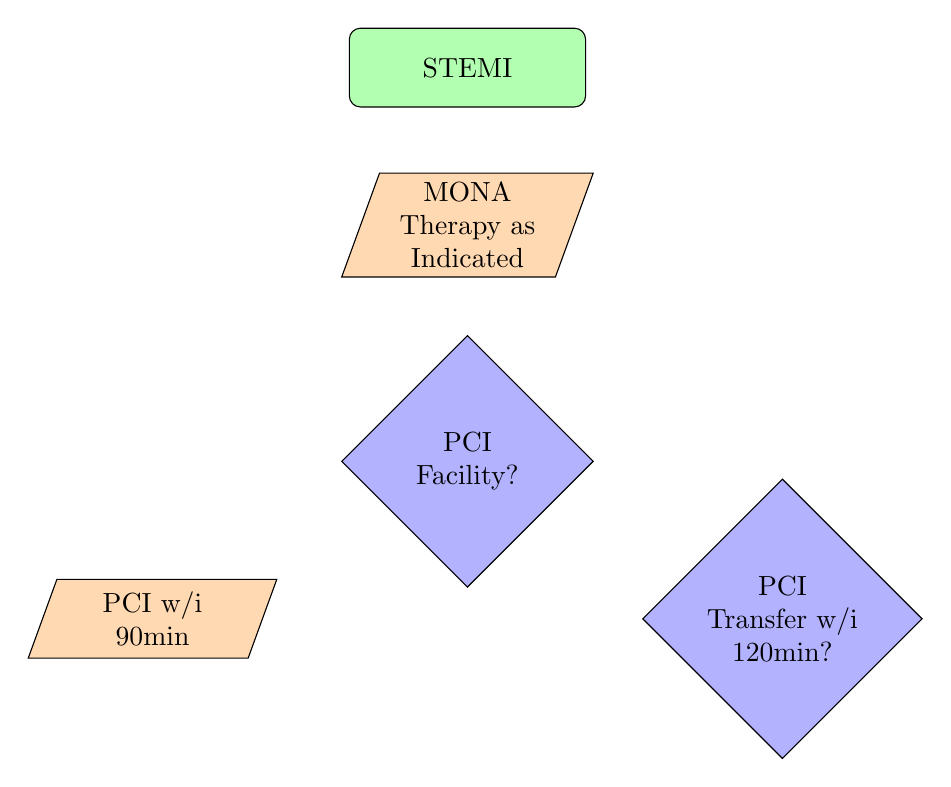
\begin{tikzpicture}[node distance=2cm]

\node [startstop] (STEMI) {STEMI};
\node [therapy, below of=STEMI] (mona) {MONA Therapy as Indicated};
\node [decision, below of=mona, yshift=-1cm] (pciAvailable) {PCI Facility?};
\node [therapy, below of=pciAvailable, xshift=-4cm] (PCI) {PCI w/i 90min};
\node [decision, below of=pciAvailable, xshift=4cm] (transfer) {PCI Transfer w/i 120min?};


\end{tikzpicture}
\end{document}